\subsection{CombinatorialDerivation}
\label{sec:CombinatorialDerivation}

The purpose of the \sbol{CombinatorialDerivation} class is to specify combinatorial biological designs without having to specify every possible design variant. For example, a \sbol{CombinatorialDerivation} can be used to specify a library of reporter gene variants that include different promoters and RBSs without having to specify a \sbol{Component} for every possible combination of promoter, RBS, and CDS in the library. \sbol{Component} objects that realize a \sbol{CombinatorialDerivation} can be derived in accordance with the class properties \sbol{template}, \\
\sbol{hasVariableComponent}, and \sbol{strategy} (see \ref{uml:combinatorial_derivation}).

\begin{figure}[ht]
\begin{center}
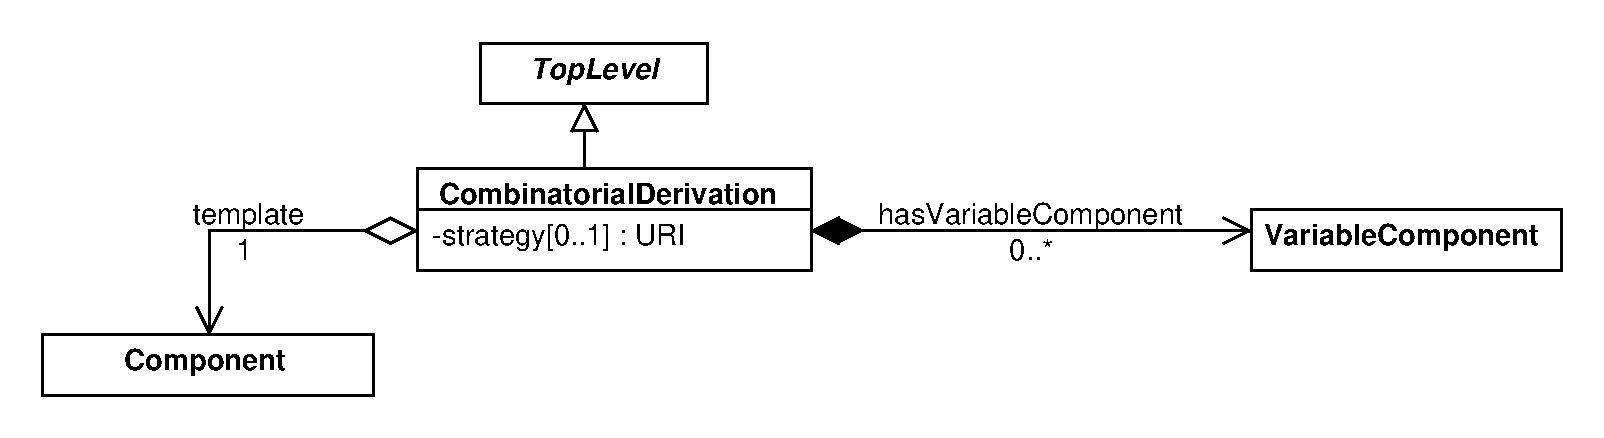
\includegraphics[scale=0.6]{uml/combinatorial_derivation}
\caption[]{Diagram of the \sbol{CombinatorialDerivation} class and its associated properties.}
\label{uml:combinatorial_derivation}
\end{center}
\end{figure}

\subparagraph{The \sbolheading{template} property}\label{sec:template}

The \sbol{template} property is REQUIRED and MUST contain a URI that refers to a \sbol{Component}. 
This \sbol{Component} is expected to serve as a template for the derivation of new \sbol{Component} objects. 
Consequently, its \sbol{hasFeature} properties SHOULD contain one or more \sbol{SubComponent} objects that describe its substructure (referred to hereafter as template \sbol{SubComponent} objects), and its \sbol{hasConstraint} property MAY also contain one or more \sbol{Constraint} objects that constrain this substructure.

When a \sbol{Component} is derived in accordance with a \sbol{CombinatorialDerivation}, the \prov{wasDerivedFrom} property of the derived \sbol{Component} SHOULD refer to the \sbol{CombinatorialDerivation}. When multiple \sbol{Component} objects are derived in accordance with the same \sbol{CombinatorialDerivation}, they MAY be referred to by the \sbol{member} property of a \sbol{Collection}, in which case the \prov{wasDerivedFrom} property of the \sbol{Collection} SHOULD also refer to this \sbol{CombinatorialDerivation}.

If the \sbolmult{type:C}{type} property of the template \sbol{Component} contains one or more URIs, then the \sbolmult{type:C}{type} property of any derived \sbol{Component} SHOULD also contain those URIs. 
The same holds true for the \sbolmult{role:C}{role} properties of these \sbol{Component} objects.

\subparagraph{The \sbolheading{hasVariableComponent} property}\label{sec:hasVariableComponent}

Each \sbol{VariableComponent} child of a \sbol{CombinatorialDerivation} defines the set of possible values for one of the variables in the \sbol{template}.
A \sbol{CombinatorialDerivation} object can have zero or more \sbol{hasVariableComponent} properties, each of type \sbol{URI}, specifying a \sbol{VariableComponent}. 
The set of  \sbol{hasVariableComponent} properties MUST NOT contain two or more \sbol{VariableComponent} objects that refer to the same template \sbol{SubComponent} via their \sbol{variable} properties (i.e., do not define the same variable twice).

The \sbol{variable} properties of \sbol{VariableComponent} objects control which \sbol{SubComponent} objects in the \sbol{template} are modified in a derived \sbol{Component}.
If no \sbol{variable} property of one of these \sbol{VariableComponent} objects refers to a template \sbol{SubComponent}, then it is not a variable and the derived object SHOULD have a \sbol{SubComponent} with identical \sbol{instanceOf} and \sbol{sourceLocation} properties
and a \prov{wasDerivedFrom} property that refers to the template \sbol{SubComponent}.

If a \sbol{SubComponent} in the \sbol{template} is referred to by some \sbol{variable} in a \sbol{VariableComponent}, then it is a variable and it SHOULD be replaced in the derived \sbol{Component} by a number of \sbol{SubComponent} objects constrained by the number specified by the \sbol{cardinality} property of the \sbol{VariableComponent} (see \ref{tbl:cardinality}).
Each \sbol{instanceOf} property of such a \sbol{SubComponent} object in the derived \sbol{Component} MUST refer to a \sbol{Component} object specified by a \sbol{variant}, contained within a \sbol{variantCollection}, or derived from a \sbol{variantDerivation} of the \sbol{VariableComponent}.


Finally, all derived \sbol{SubComponent} objects MUST follow the \sbol{restriction} properties of any 
\sbol{Constraint} objects that refer to their corresponding template \sbol{SubComponent}, and SHOULD have values of \sbolmult{role:F}{role} that contain the same values as the \sbolmult{role:F}{role} in the template \sbol{SubComponent}.


\subparagraph{The \sbolheading{strategy} property}\label{sec:strategy}
The \sbol{strategy} property is OPTIONAL and has a data type of URI. \ref{tbl:strategy} provides a list of REQUIRED \sbol{strategy} URIs. If the \sbol{strategy} property is not empty, then it MUST contain a URI from \ref{tbl:strategy}. This property recommends how many \sbol{Component} objects SHOULD be derived from the template \sbol{Component}.

\begin{table}[ht]
  \begin{edtable}{tabular}{lp{4in}}
    \toprule
    \textbf{Strategy URI} & \textbf{Description} \\
    \midrule
    \url{http://sbols.org/v2#enumerate}  &  Derivation SHOULD produce all possible \sbol{Component} objects specified by the \sbol{CombinatorialDerivation}. \\
        \url{http://sbols.org/v2#sample}  & Derivation SHOULD produce a subset of possible \sbol{Component} objects specified by \sbol{CombinatorialDerivation}. The manner in which this subset is chosen is left unspecified. \\
    \bottomrule
  \end{edtable}
  \caption{REQUIRED \sbol{URI}s for the \sbol{strategy} property.}
  \label{tbl:strategy}
\end{table}

\subsubsection{VariableComponent}
\label{sec:VariableComponent}

As described \sbolmult{hasVariableComponent}{above}, the \sbol{VariableComponent} class specifies a variable and set of values that will replace one of the \sbol{SubComponent} objects in the \sbol{template} of a \sbol{CombinatorialDerivation}.
The variable is specified by the \sbol{variable} property,
and the set of values is defined by the union of \sbol{Component} objects referred to by the \sbol{variant}, \sbol{variantCollection}, and \sbol{variantDerivation} properties.

Note that this union is intended to be a set and not a multi-set.
For example, if the \sbol{variant} property contains a \sbol{Component} $A$ and the \sbol{variantCollection} property has a \sbol{Collection} containing both \sbol{Component} $A$ and  \sbol{Component} $B$, then $A$ SHOULD NOT be selected twice during enumeration, and it SHOULD NOT be selected twice as much as $B$ during sampling.

\begin{figure}[ht]
\begin{center}
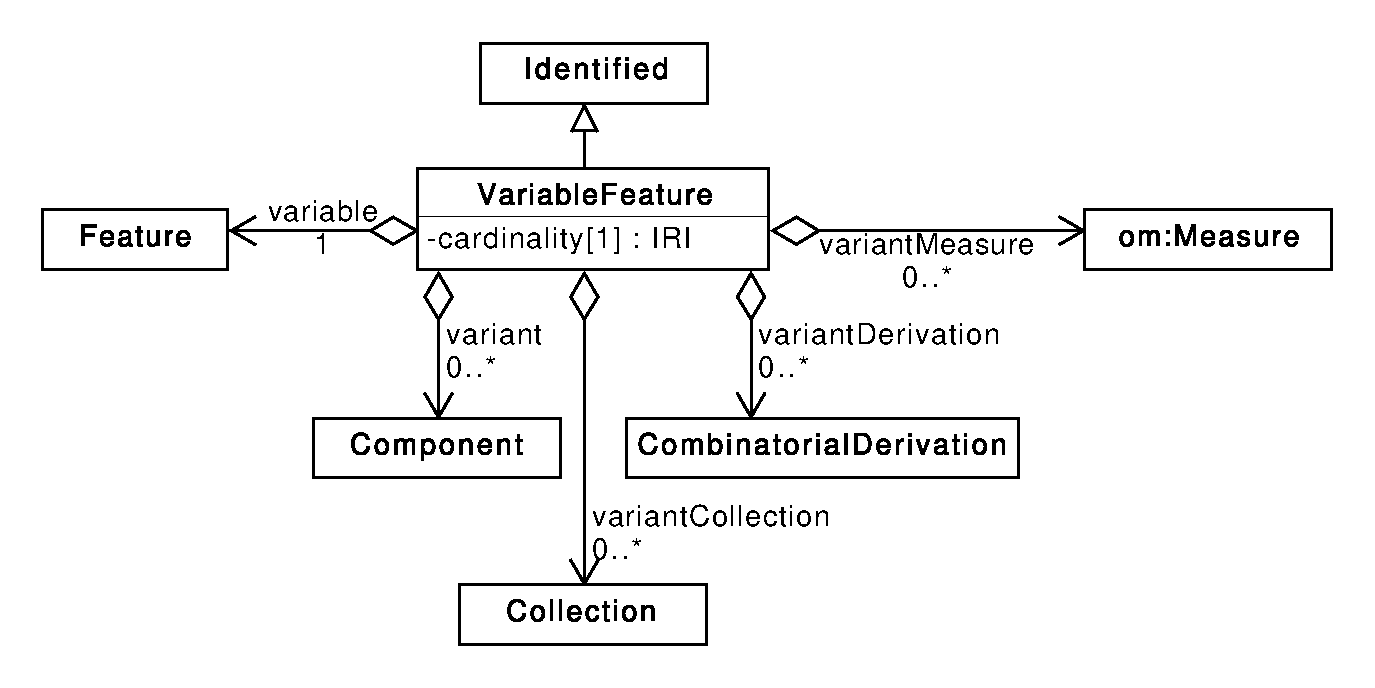
\includegraphics[scale=0.6]{uml/variable_component}
\caption[]{Diagram of the \sbol{VariableComponent} class and its associated properties.}
\label{uml:variable_component}
\end{center}
\end{figure}

\subparagraph{The \sbolheading{variable} property}\label{sec:variable}

The \sbol{variable} property is REQUIRED and MUST contain a URI that refers to a template \sbol{SubComponent} in the \sbol{template} \sbol{Component} referred to by this \sbol{VariableComponent}'s parent \sbol{CombinatorialDerivation}

\subparagraph{The \sbolheading{variant} property}\label{sec:variant}

A \sbol{VariableComponent} object can have zero or more \sbol{variant} properties, each of type \sbol{URI}, specifying a \sbol{Component} object. This property specifies individual \sbol{Component} objects to serve as options when deriving a new
\sbol{SubComponent} for the \sbol{variable} \sbol{SubComponent} from the \sbol{template}.

\subparagraph{The \sbolheading{variantCollection} property}\label{sec:variantCollection}

A \sbol{VariableComponent} object can have zero or more \sbol{variantCollection} properties, each of type \sbol{URI}, specifying a \sbol{Collection} object.
Such a \sbol{Collection} MUST NOT contain any objects besides \sbol{Component} objects or \sbol{Collection} objects that themselves contain only \sbol{Component} or \sbol{Collection} objects.
This property enables the specification of existing groups of \sbol{Component} objects to serve as options.

\subparagraph{The \sbolheading{variantDerivation} property}\label{sec:variantDerivation}

A \sbol{VariableComponent} object can have zero or more \sbol{variantDerivation} properties, each of type \sbol{URI}, specifying a \sbol{CombinatorialDerivation} object. 
This property enables the specification of \sbol{Component} objects derived in accordance with another \sbol{CombinatorialDerivation} to serve as options when deriving a new \sbol{SubComponent} for the \sbol{variable} \sbol{SubComponent} from the \sbol{template}. 
The \sbol{variantDerivation} properties of a \sbol{VariableComponent} MUST NOT refer to the \sbol{CombinatorialDerivation} that contains this \sbol{VariableComponent}. 
Furthermore, such \sbol{VariableComponent} objects MUST NOT form a cyclical chain of references via their \sbol{variantDerivation} properties and the \sbol{CombinatorialDerivation} objects that contain them. 

\subparagraph{The \sbolheading{cardinality} property}\label{sec:cardinality}

The \sbol{cardinality} property is REQUIRED and has type of URI. This property specifies how many \sbol{SubComponent} objects SHOULD be derived from the template \sbol{SubComponent} during the derivation of a new \sbol{Component}. The URI value of this property MUST come from the URIs provided in~\ref{tbl:cardinality}.

\begin{table}[ht]
  \begin{edtable}{tabular}{lp{4in}}
    \toprule
    \textbf{Cardinality URI} & \textbf{Description} \\
    \midrule
    \url{http://sbols.org/v2#zeroOrOne} & No more than one \sbol{SubComponent} in the derived \sbol{Component} SHOULD have a \prov{wasDerivedFrom} property that refers to the template \sbol{SubComponent}. \\
        \url{http://sbols.org/v2#one} & Exactly one \sbol{SubComponent} in the derived \sbol{Component} SHOULD have a \prov{wasDerivedFrom} property that refers to the template \sbol{SubComponent}. \\
\url{http://sbols.org/v2#zeroOrMore} & Any number of \sbol{SubComponent} objects in the derived \sbol{Component} MAY have \prov{wasDerivedFrom} properties that refer to the template \sbol{SubComponent}. \\
\url{http://sbols.org/v2#oneOrMore} & At least one \sbol{SubComponent} in the derived \sbol{Component} SHOULD have a \prov{wasDerivedFrom} property that refers to the template \sbol{SubComponent}. \\
    \bottomrule
  \end{edtable}
  \caption{REQUIRED \sbol{URI}s for the \sbol{cardinality} property.}
  \label{tbl:cardinality}
\end{table}

